% Konfusionsmatrix als Vektorgrafik. Übersetzen mit: pdflatex confusion_matrix.tex
\documentclass[tikz,border=4pt]{standalone}
\usepackage[T1]{fontenc}
\usepackage[utf8]{inputenc}
\usepackage{lmodern}
\renewcommand{\familydefault}{\sfdefault}
\definecolor{dunkel}{RGB}{33,95,154}   % Blau der übrigen Diagramme
\definecolor{hell}{RGB}{222,233,245}
\begin{document}
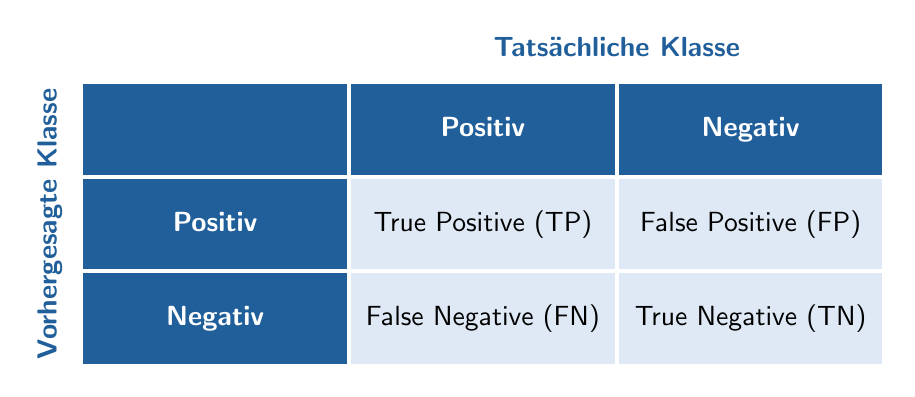
\begin{tikzpicture}[
    x=3.4cm, y=1.2cm,
    every node/.append style={text height=1.6ex, text depth=0.4ex},
    kopf/.style={draw=white, line width=1.5pt, fill=dunkel, text=white, font=\bfseries,
                 minimum width=3.4cm, minimum height=1.2cm},
    zelle/.style={draw=white, line width=1.5pt, fill=hell, text=black,
                  minimum width=3.4cm, minimum height=1.2cm}]
  % Achsenbeschriftungen
  \node[text=dunkel, font=\bfseries] at (1.5, 0.85) {Tatsächliche Klasse};
  \node[text=dunkel, font=\bfseries, rotate=90] at (-0.62, -1) {Vorhergesagte Klasse};
  % Kopfzeile
  \node[kopf] at (0, 0) {};
  \node[kopf] at (1, 0) {Positiv};
  \node[kopf] at (2, 0) {Negativ};
  % Zeilen
  \node[kopf]  at (0, -1) {Positiv};
  \node[zelle] at (1, -1) {True Positive (TP)};
  \node[zelle] at (2, -1) {False Positive (FP)};
  \node[kopf]  at (0, -2) {Negativ};
  \node[zelle] at (1, -2) {False Negative (FN)};
  \node[zelle] at (2, -2) {True Negative (TN)};
\end{tikzpicture}
\end{document}
